\documentclass[journal=jacsat,manuscript=article]{achemso}

\usepackage[version=3]{mhchem} 	% Formula subscripts using \ce{}
\usepackage{graphicx}
\graphicspath{{figure/}}		%FOLDER PATH for FIGURE
\usepackage[T1]{fontenc} 		% Use modern font encodings
\usepackage{siunitx}
\usepackage{chemformula}
\DeclareSIUnit\Molar{\textsc{m}}
% !TeX root = ./efcs.tex
\usepackage{xr} 
\externaldocument{Sup_info}
%======================New command========================
\newcommand{\uW}{\ensuremath{\,\mu\textrm{W}}}
\newcommand{\nm}{\ensuremath{\,\textrm{nm}}}
\newcommand{\uM}{\ensuremath{\,\mu\textrm{M}}}
\newcommand{\mm}{\ensuremath{\,\textrm{mm}}}
%======================Author information====================== 
\author{Biswajit Pradhan}
\affiliation[Leiden University]
{Huygens-Kamerlingh Onnes Laboratory, Leiden University, RA, Leiden, The Netherlands}
\author{Saumyakanti Khatua}
\affiliation{Department of Chemistry, IIT-Gandhinagar, Ahmedabad - 382424, India}
\author{Ankur Gupta}
\affiliation{Department of Chemistry, IISER Bhopal, 462066, Madhya Pradesh, India}

\author{Thijs Aartsma}
\author{Gerard Canters}
\author{Michel Orrit}
\affiliation[Leiden University]
{Huygens-Kamerlingh Onnes Laboratory, Leiden University, 2300 RA Leiden, Netherlands}
\email{orrit@physics.leidenuniv.nl}
\phone{+31 (0)71 527 1720}
\title[]
{Gold-Nanorod-Enhanced FCS of Fluorophores with High Quantum Yield in Lipid Bilayers}

\abbreviations{FCS}
\keywords{American Chemical Society, \LaTeX}
%%%%%%%%%%%%%%%%%%%%%%%%%%%%%%%%%%%%%%%%%%%%%%%%%%%%%%%%%%%%%%%%%%
%%%%%%% Start the main part of the manuscript here.%%%%%%%%%%%%%%
%%%%%%%%%%%%%%%%%%%%%%%%%%%%%%%%%%%%%%%%%%%%%%%%%%%%%%%%%%%%%%%%%%
\begin{document}
\begin{abstract}
	Plasmonic fluorescence enhancement is used to study fluorescence correlation spectroscopy (FCS) at higher concentrations than in regular diffraction-limited FCS experiments. Previous studies suffered from sticking to the substrate and were performed mainly with poorly emitting dyes. A lipid bilayer forms a passivating surface preventing sticking of the dye or the protein and allows for specific anchoring of probe molecules. For dyes with high quantum yields, the fluorescence background of unenhanced molecules is high, and the fluorescence enhancement is weak, less than about 10. Nonetheless, we show that FCS is possible at micromolar concentrations of the probe molecule. Enhanced FCS is recorded by selecting signals on the basis of their shortened lifetime. This selection enhances the contrast of the correlation by more than an order of magnitude. The lipid bilayer can be used to anchor biomolecules and perform enhanced FCS, as we show for a dye-labeled protein.
\end{abstract}
\pagebreak
%============================Introduction=====================================
Fluorescence-based single-molecule detection helps exploring the structure and dynamics of complex biological matter.\cite{moerner1999illuminating,weiss1999fluorescence} Single-molecule signals can reveal a transient state during a chemical reaction, or report on the kinetics of processes as a function of position. Broadly there are two ways of studying single molecules: i) by immobilizing the molecule on a backgroundfree matrix or surface, ii) by dissolving the molecules in a fluid and measuring the signal fluctuation by fluorescence correlation spectroscopy (FCS).\cite{Magde1972} Both techniques require the molecule to possess a high quantum yield and good photostability. FCS studies are limited to concentrations in the pico- to nano-molar range, in view of the diffraction-limited detection volume of a few femtoliters (fL). As many biological reactions occur in the micromolar range4, smaller detection volumes are desirable to study these reactions by FCS.\\

Plasmonic nanostructures can both enhance molecular fluorescence in volumes smaller than the diffraction-limited volume and reduce the background fluorescence of the other molecules in the diffraction-limited volume. Zero-mode waveguides and antennas-in-box, in particular, both enhance fluorescence and reduce background.\cite{levene2003zeromode,kinkhabwala2012fluorescence,punj2013a,yuan2013thousandfold,punj2013gold} The effective fluorescence enhancement depends sensitively on the position and orientation of the molecule with respect to the nanoparticle. It originates from two factors, excitation enhancement and radiative enhancement. By confining the optical field into so-called hot spots with volumes much smaller than the diffraction limit,\cite{schuller2010plasmonics} plasmonic nanostructures enhance the incident field by up to a few orders of magnitude, leading to excitation enhancement.\cite{yuan2013thousandfold,anger2006enhancement,kinkhabwala2009large,acuna2012fluorescence,busson2012accelerated,holzmeister2014quantum,khatua2014resonant} They also alter the radiative and non-radiative decay rates of molecules in their vicinity. The ensuing radiative enhancement results from improved emission by the nanoantenna dipole induced by the molecular dipole. In addition, energy may be transferred from the molecule to the antenna resulting in non-radiative losses and energy dissipation in the metal. Changes in the radiative or non-radiative decay paths lead to altered, generally shortened fluorescence lifetimes.\cite{khatua2014resonant,liu2007quantized,lakowicz2001radiative,dulkeith2005gold,seelig2007nanoparticleinduced,muskens2007strong,pelton2015modified} Distance-dependent lifetime measurements show lifetime shortening up to 40 nm away from the metal surface.\cite{seelig2007nanoparticleinduced}\\

Noble-metal plasmonic nanostructures can be fabricated either by lithography or by colloid chemistry.\cite{zijlstra2011single} Whereas lithography can produce nanostructures with arbitrary geometries suitable for high optical confinement, it presents the disadvantages of complex processing, polycrystallinity, surface roughness, and high cost. Colloidal chemistry produces large numbers of highly crystalline nanostructures in a few basic shapes (spheres, rods, bipyramids, etc.) that are controllable to some extent, at a low cost. Among the basic nanoparticle shapes, nanorods\cite{yuan2013thousandfold} can be just as efficient as lithographically-made structures\cite{punj2013a,kinkhabwala2009large} in enhancing fluorescence. Gold nanorods confine the optical field more weakly than lithographically made gap structures, but they have the advantage of a narrow surface plasmon resonance, which can be tuned in the red and near infrared range by changing the rod’s aspect ratio.\cite{khatua2014resonant} The largest enhancement is achieved for a maximum overlap of the molecule’s excitation and fluorescence spectra, of the nanorod’s surface plasmon resonance, and of the excitation wavelength. Further advantages of gold nanoparticles are that they provide easy access of hot spots to diffusing molecules and that they can be inserted into complex environments such as living cells.\\

Confinement of light in volumes much smaller than the diffraction-limited volume combined with fluorescence enhancement open applications of FCS at micromolar dye concentrations. The correlation contrast in FCS decays as the square of the background intensity. To reduce background, most enhanced FCS experiments have been done on dyes with low quantum yields.\cite{kinkhabwala2012fluorescence,estrada200810000} Alternatively, a fluorescence quencher may be added to a dye with a high quantum yield (QY) to reduce background.\cite{punj2013a,punj2013gold} A metal box or cladding\cite{ghenuche2015matching} can also be fabricated around the nano structure to improve the correlation contrast against the background of unenhanced molecules. Both solutions have disadvantages, as a millimolar quencher concentration may be harmful to a living cell. Metal claddings are difficult to fabricate and to manipulate in a complex environment. Generalizing enhanced FCS to high-QY dyes would obviate these two problems and open plasmonic enhancement to biological marker dyes, most of which have high QY. Plasmonic enhancement may also help overcome other background sources such as autofluorescence in live-cell experiments. Indeed, as we show herein, even weak fluorescence enhancements suffice to overcome background in FCS experiments. Moreover, fluorescence photons with short emission times may be selected as was done by Acuna et al\cite{acuna2012fluorescence} further to improve the signal to noise ratio of enhanced FCS.\\

A further limitation in working with metal nanostructures on a solid substrate is the nonspecific interaction of the molecules with metal and substrate, which not only may affect the molecules’ functionality but also make measurements troublesome.\cite{kinkhabwala2012fluorescence,yuan2013thousandfold,zhang2009gold} Micellar solutions have been used to minimize sticking but are not ideal when studying biomolecules or performing experiments in live cells. We therefore need to suppress or mitigate nonspecific interactions of the dyes or biomolecules under study with the solid substrates supporting the structures. Living organisms use a lipid bilayer on their outer surface to prevent nonspecific interaction and protein fouling while allowing specific binding of membrane proteins.\cite{zhang2009gold,cooper2000cell} We have used a supported lipid bilayer to passivate the substrate.\cite{persson2012lipidbased,ller2012single,lohmuller2011supported} Supported bilayer can be self-assembled on solid surfaces (glass, silica, and similar polar surfaces) such that it forms a single, continuous membrane which possesses a high degree of lateral mobility by maintaining a very thin layer of water (1~nm) between substrate and bilayer.\cite{sackmann1996supported,CASTELLANA2006429,cremer1999formation,richter2006formation} Bilayers are also model systems to study diffusion in biological membranes. In standard experiments, diffusion in bilayers is studied on length scales limited by far-field resolution. Plasmonic enhancement gives us access to diffusion on the length scales of the near field, typically some tens of nm. Enhanced fluorescence experiments provide access to nanoscale diffusion in the vicinity of a gold nanorod.\\

Here we study fluorescence enhancement of a high-QY dye by immobilized single gold nanorods. Sticking of the dye to the glass substrate was prevented by coating the glass with a supported lipid bilayer formed from a zwitterionic lipid. We have characterized the properties of the enhanced signal and shown that its fluorescence decay is much faster than the far-field signal’s. Based on these time decay characteristics, we have filtered the near-field signal from the background of unenhanced dye fluorescence, thereby obtaining an improved FCS contrast. The same measurement provides both far-field and near-field diffusion components, and allows us to compare the diffusion kinetics in both regimes. We show that biomolecules can be successfully anchored in the bilayer, and that enhanced FCS can be performed while sticking and interaction with gold nanorods are prevented.\\
\begin{figure}
	\centering
	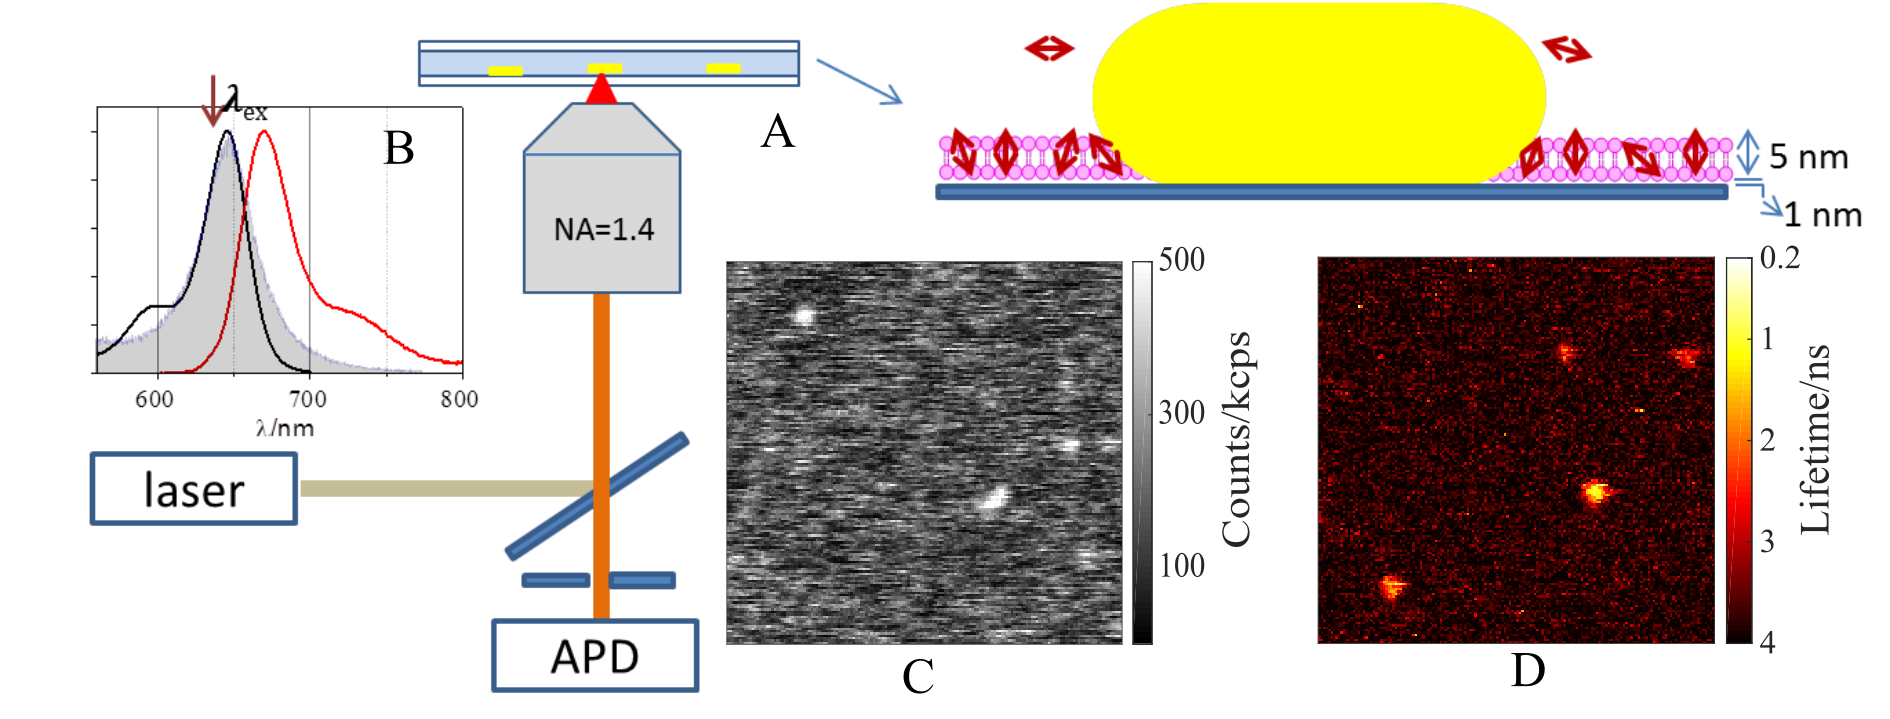
\includegraphics[width=\textwidth]{schematic.png}
	\caption{(A) Schematic diagram of the optical setup with a supported lipid bilayer (pink), ATTO 647N molecules (red) and a gold nanorod (yellow). (B) Absorption spectrum of ATTO 647N (black), fluorescence spectrum of ATTO 647N (red) and photoluminescence spectrum of a single gold nanorod (shaded area). Notice the overlap of the nanorod's SPR with the dye's absorption and emission spectra. (C) fluorescence intensity image (size $8~\uW \times 8~\uW$) and (D) fluorescence lifetime image (FLIM) of the same area of lipid bilayer. Note the lack of correlation between the fluorescent spots indicating dye aggregates in (C) and the short-lifetime spots in (D) indicating the rods.}
	\label{fig:schematic}
\end{figure}
%===========================Methods================================
\section{METHODS}
\subsection{Gold nanorod immobilization}
Gold nanorods (AuNRs) were synthesized in cetyl trimethyl ammonium bromide (CTAB) using the seed-mediated growth method.\cite{nikoobakht2003preparation} The average dimension of the nanorods was $90~\nm\times50~\nm$. Fig. S1B shows a scanning electron microscopy image of the nanoparticles. The bulk absorption spectra of these nanorods in Fig.S1A show the longitudinal surface plasmon resonance (LSPR) at 640 nm. The nanorod sample was diluted and the CTAB was washed away by centrifugation and re-suspension in milliQ water before use. Glass coverslips (Menzel-Glaser, 22 mm × 40 mm, no. 1 thickness) were used for immobilization. The coverslips were sonicated in water (15 min) and acetone (15 min). Then they were rinsed in milliQ water several times and incubated in a H2O/NH4OH/H2O2 (5:1:1) bath at 70 0C. The coverslips were rinsed several times with water and ethanol, and finally stored in ethanol. Before use the coverslips were flamed, and then ozone-cleaned for 15 minutes. The nanorods were spin-coated onto these coverslips at 2,000 rpm for 1 minute. These parameters gave us around 5 particles per 100 μm2 area and more than 90\% of them were single. The coverslips with the gold nanorods were then rinsed with water to remove remaining traces of CTAB, dried, and again ozone-cleaned for 30 minutes. This resulted in a very  hydrophilic surface. The coverslip was mounted in a homemade flow cell, where the surface was further prepared for confocal experiments.
% \bibliographystyle{achemso.bst}
\bibliography{efcs}
\end{document}